\documentclass[c]{beamer}
% Этот шаблон документа разработан в 2014 году
% Данилом Фёдоровых (danil@fedorovykh.ru) 
% для использования в курсе 
% <<Документы и презентации в \LaTeX>>, записанном НИУ ВШЭ
% для Coursera.org: http://coursera.org/course/latex .
% Исходная версия шаблона --- 
% https://www.writelatex.com/coursera/latex/5.3

% В этом документе преамбула

\usepackage{siunitx}
%%% Работа с русским языком
%\usepackage{cmap}					% поиск в PDF
%\usepackage{mathtext} 				% русские буквы в формулах
%\usepackage[T2A]{fontenc}			% кодировка
%\usepackage[utf8]{inputenc}			% кодировка исходного текста
%\usepackage[english,russian]{babel}	% локализация и переносы
%\usepackage{indentfirst}
%\frenchspacing
%
%\renewcommand{\epsilon}{\ensuremath{\varepsilon}}
%\newcommand{\phibackup}{\ensuremath{\phi}}
%\renewcommand{\phi}{\ensuremath{\varphi}}
%\renewcommand{\varphi}{\ensuremath{\phibackup}}
%\renewcommand{\kappa}{\ensuremath{\varkappa}}
%\renewcommand{\le}{\ensuremath{\leqslant}}
%\renewcommand{\leq}{\ensuremath{\leqslant}}
%\renewcommand{\ge}{\ensuremath{\geqslant}}
%\renewcommand{\geq}{\ensuremath{\geqslant}}
%\renewcommand{\emptyset}{\varnothing}
%\renewcommand{\Im}{\operatorname{Im}}
%\renewcommand{\Re}{\operatorname{Re}}


%%% Дополнительная работа с математикой
\usepackage{amsmath,amsfonts,amssymb,amsthm,mathtools} % AMS
%\usepackage{icomma} % "Умная" запятая: $0,2$ --- число, $0, 2$ --- перечисление

%% Номера формул
%\mathtoolsset{showonlyrefs=true} % Показывать номера только у тех формул, на которые есть \eqref{} в тексте.
%\usepackage{leqno} % Нумереация формул слева

%% Свои команды
\DeclareMathOperator{\sgn}{\mathop{sgn}}
\DeclareMathOperator{\sign}{\mathop{sign}}
\DeclareMathOperator*{\res}{\mathop{res}}
\DeclareMathOperator*{\tr}{\mathop{tr}}
\DeclareMathOperator*{\rot}{\mathop{rot}}
\DeclareMathOperator*{\divop}{\mathop{div}}
\DeclareMathOperator*{\grad}{\mathop{grad}}

%% Перенос знаков в формулах (по Львовскому)
\newcommand*{\hm}[1]{#1\nobreak\discretionary{}
{\hbox{$\mathsurround=0pt #1$}}{}}

%%% Работа с картинками
\usepackage{graphicx}  % Для вставки рисунков
\graphicspath{{figures/}}  % папки с картинками
\setlength\fboxsep{3pt} % Отступ рамки \fbox{} от рисунка
\setlength\fboxrule{1pt} % Толщина линий рамки \fbox{}
\usepackage{wrapfig} % Обтекание рисунков текстом

%%% Работа с таблицами
\usepackage{array,tabularx,tabulary,booktabs} % Дополнительная работа с таблицами
\usepackage{longtable}  % Длинные таблицы
\usepackage{multirow} % Слияние строк в таблице

%%% Теоремы
\theoremstyle{plain} % Это стиль по умолчанию, его можно не переопределять.
\newtheorem{thm}{Теорема}
\newtheorem*{thm*}{Теорема}
\newtheorem{prop}{Предложение}
\newtheorem*{prop*}{Предложение}
 
\theoremstyle{definition} % "Определение"
%\newtheorem{corollary}{Следствие}[theorem]
\newtheorem{dfn}{Определение}
\newtheorem*{dfn*}{Определение}
\newtheorem{prob}{Задача}
\newtheorem*{prob*}{Задача}

 
\theoremstyle{remark} % "Примечание"
\newtheorem*{sol}{Решение}
\newtheorem*{rem}{Замечание}

%%% Программирование
\usepackage{etoolbox} % логические операторы

%%% Страница
%\usepackage{extsizes} % Возможность сделать 14-й шрифт
%\usepackage{geometry} % Простой способ задавать поля
%	\geometry{top=25mm}
%	\geometry{bottom=35mm}
%	\geometry{left=35mm}
%	\geometry{right=20mm}
 
\usepackage{fancyhdr} % Колонтитулы
%	\pagestyle{fancy}
 %	\renewcommand{\headrulewidth}{0pt}  % Толщина линейки, отчеркивающей верхний колонтитул
	%\lfoot{Нижний левый}
	%\rfoot{Нижний правый}
	%\rhead{Верхний правый}
	%\chead{Верхний в центре}
	%\lhead{Верхний левый}
	%\cfoot{Нижний в центре} % По умолчанию здесь номер страницы

\usepackage{setspace} % Интерлиньяж
%\onehalfspacing % Интерлиньяж 1.5
%\doublespacing % Интерлиньяж 2
%\singlespacing % Интерлиньяж 1

\usepackage{lastpage} % Узнать, сколько всего страниц в документе.

\usepackage{soul} % Модификаторы начертания

\usepackage{hyperref}
\usepackage[usenames,dvipsnames,svgnames,table,rgb]{xcolor}
\hypersetup{				% Гиперссылки
    unicode=true,           % русские буквы в раздела PDF
    pdftitle={Заголовок},   % Заголовок
    pdfauthor={Автор},      % Автор
    pdfsubject={Тема},      % Тема
    pdfcreator={Создатель}, % Создатель
    pdfproducer={Производитель}, % Производитель
    pdfkeywords={keyword1} {key2} {key3}, % Ключевые слова
%    colorlinks=true,       	% false: ссылки в рамках; true: цветные ссылки
    %linkcolor=red,          % внутренние ссылки
    %citecolor=black,        % на библиографию
    %filecolor=magenta,      % на файлы
    %urlcolor=cyan           % на URL
}

\usepackage{csquotes} % Еще инструменты для ссылок

%\usepackage[style=apa,maxcitenames=2,backend=biber,sorting=nty]{biblatex}

\usepackage{multicol} % Несколько колонок

\usepackage{tikz} % Работа с графикой
\usepackage{pgfplots}
\usepackage{pgfplotstable}
%\usepackage{coloremoji}
\usepackage{floatrow}
\usepackage{subcaption}
\graphicspath{{figures/}}

\renewcommand\thesubfigure{\asbuk{subfigure}}
%\addbibresource{master.bib}

\usepackage{import}
\usepackage{pdfpages}
\usepackage{transparent}
\usepackage{xcolor}
\usepackage{xifthen}

\newcommand{\incfig}[2][1]{%
    \def\svgwidth{#1\columnwidth}
    \import{./figures/}{#2.pdf_tex}
}
%\usepackage{titlesec}
%\titleformat{\section}{\normalfont\Large\bfseries}{}{0pt}{}
%----------------------STANDART:
%\titleformat{\chapter}[display]
%  {\normalfont\huge\bfseries}{\chaptertitlename\ \thechapter}{20pt}{\Huge}
%\titleformat{\section}{\normalfont\Large\bfseries}{\thesection}{1em}{}
%\titleformat{\subsection}
%  {\normalfont\large\bfseries}{\thesubsection}{1em}{}
%\titleformat{\subsubsection}
%  {\normalfont\normalsize\bfseries}{\thesubsubsection}{1em}{}
%\titleformat{\paragraph}[runin]
%  {\normalfont\normalsize\bfseries}{\theparagraph}{1em}{}
%\titleformat{\subparagraph}[runin]
%  {\normalfont\normalsize\bfseries}{\thesubparagraph}{1em}{}

\pdfsuppresswarningpagegroup=1
\pgfplotsset{compat=1.16}



%\setcounter{tocdepth}{1} % only parts,chapters,sections
%\titleformat{\subsection}{\normalfont\large\bfseries}{}{0em}{}
%\titleformat{\subsubsection}{\normalfont\normalsize\bfseries}{}{0em}{}

%\newcommand{\textover}[2]{\stackrel{\mathclap{\normalfont\mbox{#2}}}{#1}}

\author{Yaroslav Drachov\\
Moscow Institute of Physics and Technology}
%\author{Драчов Ярослав\\
%Факультет общей и прикладной физики МФТИ}
\newcommand{\veq}{\mathrel{\rotatebox{90}{$=$}}}
%\newcommand{\teto}[1]{\stackrel{\mathclap{\normalfont\tiny\mbox{#1}}}{\to}}
%\renewcommand{\thesubsection}{\arabic{subsection}}

%%\setcounter{secnumdepth}{0}

\definecolor{tabblue}{RGB}{30, 119, 180}
\definecolor{taborange}{RGB}{255, 127, 15}
\definecolor{tabgreen}{RGB}{45, 160, 43}
\definecolor{tabred}{RGB}{214, 38, 40}
\definecolor{tabpurple}{RGB}{148, 103, 189}
\definecolor{tabbrown}{RGB}{140, 86, 76}
\definecolor{tabpink}{RGB}{227, 119, 193}
\definecolor{tabgray}{RGB}{127, 127, 127}
\definecolor{tabolive}{RGB}{188, 189, 33}
\definecolor{tabcyan}{RGB}{22, 190, 207}
\pgfplotscreateplotcyclelist{colorbrewer-tab}{
{tabblue},
{taborange},
{tabgreen},
{tabred},
{tabpurple},
{tabbrown},
{tabpink},
{tabgray},
{tabolive},
{tabcyan},
}
\usepackage{csvsimple}
\usepackage{extarrows}
%\renewcommand{\labelenumii}{\asbuk{enumii})}
%\renewcommand{\labelenumiv}{\Asbuk{enumiv}}
%\newcommand{\prob}[1]{\subsubsection*{#1}}
\sisetup{output-decimal-marker = {,},separate-uncertainty = true,exponent-product = \cdot}

\usepackage{braket}
\usepackage{enumerate}
\usepackage{chngcntr}
%\counterwithin*{equation}{problem}
%\usepackage{bbold}

\newtheoremstyle{hiProb}% ⟨name ⟩ 
{3pt}% ⟨Space above ⟩1 
{3pt}% ⟨Space below ⟩1
{}% ⟨Body font ⟩
{}% ⟨Indent amount ⟩2
{\bfseries}% ⟨Theorem head font⟩
{.}% ⟨Punctuation after theorem head ⟩
{.5em}% ⟨Space after theorem head ⟩3
%{\thmname{#1} \thmnote{#3}}% ⟨Theorem head spec (can be left empty, meaning ‘normal’)⟩
{\thmnote{#3}}% ⟨Theorem head spec (can be left empty, meaning ‘normal’)⟩
\theoremstyle{hiProb} % "Определение"
%\newtheorem{hiProb}{Задача}
\newtheorem{hiProb}{}
%\usepackage{mmacells}
\newcommand{\textover}[2]{\stackrel{\mathclap{\normalfont\scriptsize\mbox{#2}}}{#1}}
\usepackage{units}
\usepackage[math]{cellspace}%
\setlength\cellspacetoplimit{2pt}
\setlength\cellspacebottomlimit{2pt}

\DeclareMathAlphabet{\mathbbold}{U}{bbold}{m}{n}

\newcommand{\normord}[1]{:\mathrel{#1}:}

\usetheme{MIPT}
\newtheorem{rthm}{Теорема}
\newtheorem{rdfn}{Определение}
\newtheorem{rproof}{Доказательство}
\newtheorem{rexample}{Пример}
\title{Старшие гомотопические группы}
\subtitle{Доклад на семинар по геометрической топологии}
\author{Драчов Ярослав}
\date{\today}
\institute[МФТИ]{Московский физико-технический институт}
\begin{document}

\frame[plain]{\titlepage}

\section{Фундаментальная группа $\pi_1(X)$}
\subsection{Путь и гомотопия путей}

\begin{frame}
\frametitle{\insertsection}
\framesubtitle{\insertsubsection}
\begin{rdfn}
	\emph{Путём} в пространстве $X$ называют непрерывное отображение
	$f\colon I\to X $, где $I$ --- это единичный интервал
	$[0,\,1]$. \emph{Петлёй} с \emph{базовой точкой} $x_0$
	называется путь, для которого
	$f(0)=f(1)=x_0 \in X$.
\end{rdfn}

\begin{rdfn}<2>
	\emph{Гомотопия путей} в $X$ --- это семейство отображений
	$f_t \colon I \to X$, $0 \le t \le 1$, таких, что
	\begin{enumerate}
		\item Конечные точки $f_t(0)=x_0$ и $f_t(1)=x_1$
		не зависят от $t$.
		 \item Связанное отображение $F \colon I\times
			 I\to X$ определённое соотношением
			 $F(s,\,t)=f_t (s)$ --- непрерывно.
	\end{enumerate}
\end{rdfn}
\end{frame}
\subsection{Определение}
\begin{frame}
\frametitle{\insertsection}
\framesubtitle{\insertsubsection}
	\begin{rdfn}
	\emph{Фундаментальной группой $\pi_1 (X,\,x_0)$} мы называли
	группу классов гомотопической эквивалентности петель с операцией умножения
	$[f][g]=[f\cdot g]$, где 
	 \[
		 f \cdot g (s)= \begin{cases}
		f(2s), & 0\le  s\le \frac{1}{2},\\
		g(2s-1), & \frac{1}{2}\le  s \le  1.
	\end{cases}
	\] 
\end{rdfn}
\end{frame}
\section{Определение $\pi_n(X)$}
\subsection{Аналогия с  $\pi_1(X)$}
\begin{frame}
\frametitle{\insertsection}
\framesubtitle{\insertsubsection}
Можно обобщить конструкцию фундаментальной группы $\pi_1(X)$
на случай  <<$n$-мерных петель>> --- сфер $S^n$ с определённой
базовой точкой  $x_0$.
\end{frame}
\begin{frame}
\frametitle{\insertsection}
\framesubtitle{\insertsubsection}
	
Пусть $I^n$ --- единичный $n$-куб, произведение $n$ копий
интервала $[0,\,1]$. 
Граница $\partial I^n$ пространства $I^n$ --- подпространство,
состоящее из точек, с хотя бы одной координатой равной
0 или 1. 
\begin{rdfn}<2>
Для пространства $X$ с базовой точкой $x_0 \in X$,
определим $\pi_n (X,\,x_0)$ как множество гомотопических
классов отображений $f \colon (I^n,\,\partial I^n) \to 
(X,\,x_0)$, где гомотопии $f_t$ должны удовлетворять условию
$f_t(\partial I^n)=x_0$ для всех $t$. Определение
расширяется на случай $n=0$, если взять $I^0$ точкой и $\partial
I^0$ пустым множеством. Так, $\pi_0(X,\,x_0)$ --- множество
компонент связности $X$.
\end{rdfn}
%\uncover<2->{Пусть  фиксированы точки $x_0 \in S_ n$ и  $x_0 \in X$. Множество
%классов гомотопных отxб0аж ений $S_n \to X$, переводящих $a_0$ в
%$x_0$ обозначают $\pi_n(X)$. Далее покажем(?), что на множестве
%$\pixn0X) $ можно ввести группо вую структуру.}
%\begin{rdfn}<3>x0 x00         
%	Полученную группу $\pi_n(X)$ называют  \emp h{$n$-мерной
%	го мотопической группой} или  \emph{$n$xй0гомотопической
%группой}.
%\end{rdfn}
\end{frame}
\subsection{Случай $n\ge 2$}
\begin{frame}
\frametitle{\insertsection}
\framesubtitle{\insertsubsection}
\begin{rdfn}
	Если $n\ge 2$, операция суммирования в $\pi_n(X,\,x_0)$,
обобщая операцию умножения в $\pi_1$, определяется как
\[
	(f+g)(s_1,\,s_2,\ldots,\,s_n)=
	\begin{cases}
		f(2s_1,\,s_2,\ldots,\,s_n), & s_1 \in \left[ 0,\,
		\frac{1}{2}\right], \\
			g(2s_1-1,\,s_2,\ldots,\, s_n), &
			s_1 \in \left[ \frac{1}{2},\, 1 \right]. 
	\end{cases}
\] 
\end{rdfn}
\only<2->{Ясно, что эта сумма однозначно определена на гомотопических
классах. Т.\:к. только первая координата вовлечена в
операцию суммирования, такие же доводы, как и для
$\pi_1$ показывают, что $\pi_n(X,\,x_0)$ --- это группа
с постоянной функцией, отображающей $I^n$ в $x_0$, в качестве
единичного элемента и обратными элементами, задаваемыми
$-f(s_1,\,s_2,\ldots,\,s_n)=f(1-s_1,\,s_2,\ldots,s_n)$.}
\end{frame}
\section{Коммутативность $\pi_n(X)$ для $n\ge 2$}
\subsection{Аддитивная запись}
\begin{frame}
\frametitle{\insertsection}
\framesubtitle{\insertsubsection}
\alt<1>{Аддитивная запись для груповой операции используется
потому, что $\pi_n (X,\,x_0)$ --- абелевы для $n\ge 2$.
А именно, $f+g \simeq g+f$ с гомотопией, изображённой на рисунке.}{}
\begin{center}
\incfig{1}
\end{center}
\alt<2>{Гомотопия начинает с уменьшения областей определения $f$ и $g$
до меньших подкубов  $I^n$, с областью снаружи этих подкубов,
отображающихся в базовую точку.}{}
\alt<3>{После того, как это сделано,
у нас появляется возможность  переставить два подкуба куда 
угодно, пока они остаются разъединёнными, поэтому если
$n\ge 2$, они могут при такой перестановке обойти друг друга
и поменяться местами.}{}
\alt<4>{После этого  для завершения гомотопии,
области определения $f$ и $g$  могут быть расширены до их
начальных размеров. Весь этот процесс может быть проведён,
используя только координаты $s_1$ и $s_2$, оставляя остальные
координаты фиксироованными.}{}
\end{frame}
\section{Отображения $S^n\to X$}
\subsection{Суть $\pi_n(X)$}
\begin{frame}
\frametitle{\insertsection}
\framesubtitle{\insertsubsection}
Отображения $(I^n,\,\partial I^n)\to (X,\, x_0)$ --- это то же
самое, что
и отображения факторпространства $I^n / \partial I^n=S^n$ 
на $X$, переводящие базовую точку $s_0= \partial I^n / \partial I^n$ в $x_0$. Это означает, что мы можем также рассматривать 
$\pi_n(X,\,x_0)$ как гомотопические классы карт $(S^n,\,s_0)
\to (X,\,x_0)$, где гомотопии --- это отображения одного вида
$(S^n,\,s_0)\to (X,\,x_0)$. \end{frame}
\begin{frame}
\frametitle{\insertsection}
\framesubtitle{\insertsubsection}
В такой интерпретации $\pi_n (X,\,x_0)$, сумма $f+g$ --- это композиция
$S^n \xrightarrow[]{c}S^n \vee S^n \xrightarrow[]{f \vee g}X$,
где $c$ сжимает экватор $S^{n-1}$ в $S^n$ в точку и мы
выбираем базовую точку $s_0$ так, чтобы она лежала в этой
$S^{-1}$.
\begin{center}
	\incfig[0.8]{2}
\end{center}
\end{frame}
\section{Базовая точка $\pi_n(X,\,x_0)$}
\subsection{Линейно связное пространство}
\begin{frame}
\frametitle{\insertsection}
\framesubtitle{\insertsubsection}
Далее покажем, что если $X$ --- линейно связное пространство,
то для различных $x_0$ их гомотопические группы $\pi_n (X,\,x_0)$
всегда дают изоморфные группы $\pi_n(X,\,x_0)$, как и для
$\pi_1$, поэтому в таком случае разрешено написание
$\pi_n(X)$ для  $\pi_n(X,\,x_0)$.
\end{frame}
\begin{frame}
\frametitle{\insertsection}
\framesubtitle{\insertsubsection}
Дан путь $\gamma \colon I \to X$ из $x_0 = \gamma(0)$ в другую
базовую точку $x_1=\gamma(1)$, мы можем сопоставить
каждому отображению $f\colon (I^n,\,\partial I^n)\to 
(X,\,x_1)$ новое отображение $\gamma f\colon (I^n,\,\partial I^n)
\to (X,\,x_0)$ сужая область определения $f$ до меньшего
концентрического куба в $ I^n$, после чего, помещая путь $\gamma$ 
на каждом радиальном сегменте оболочки между этим меньшим кубом
и $\partial I^n$.
\begin{center}
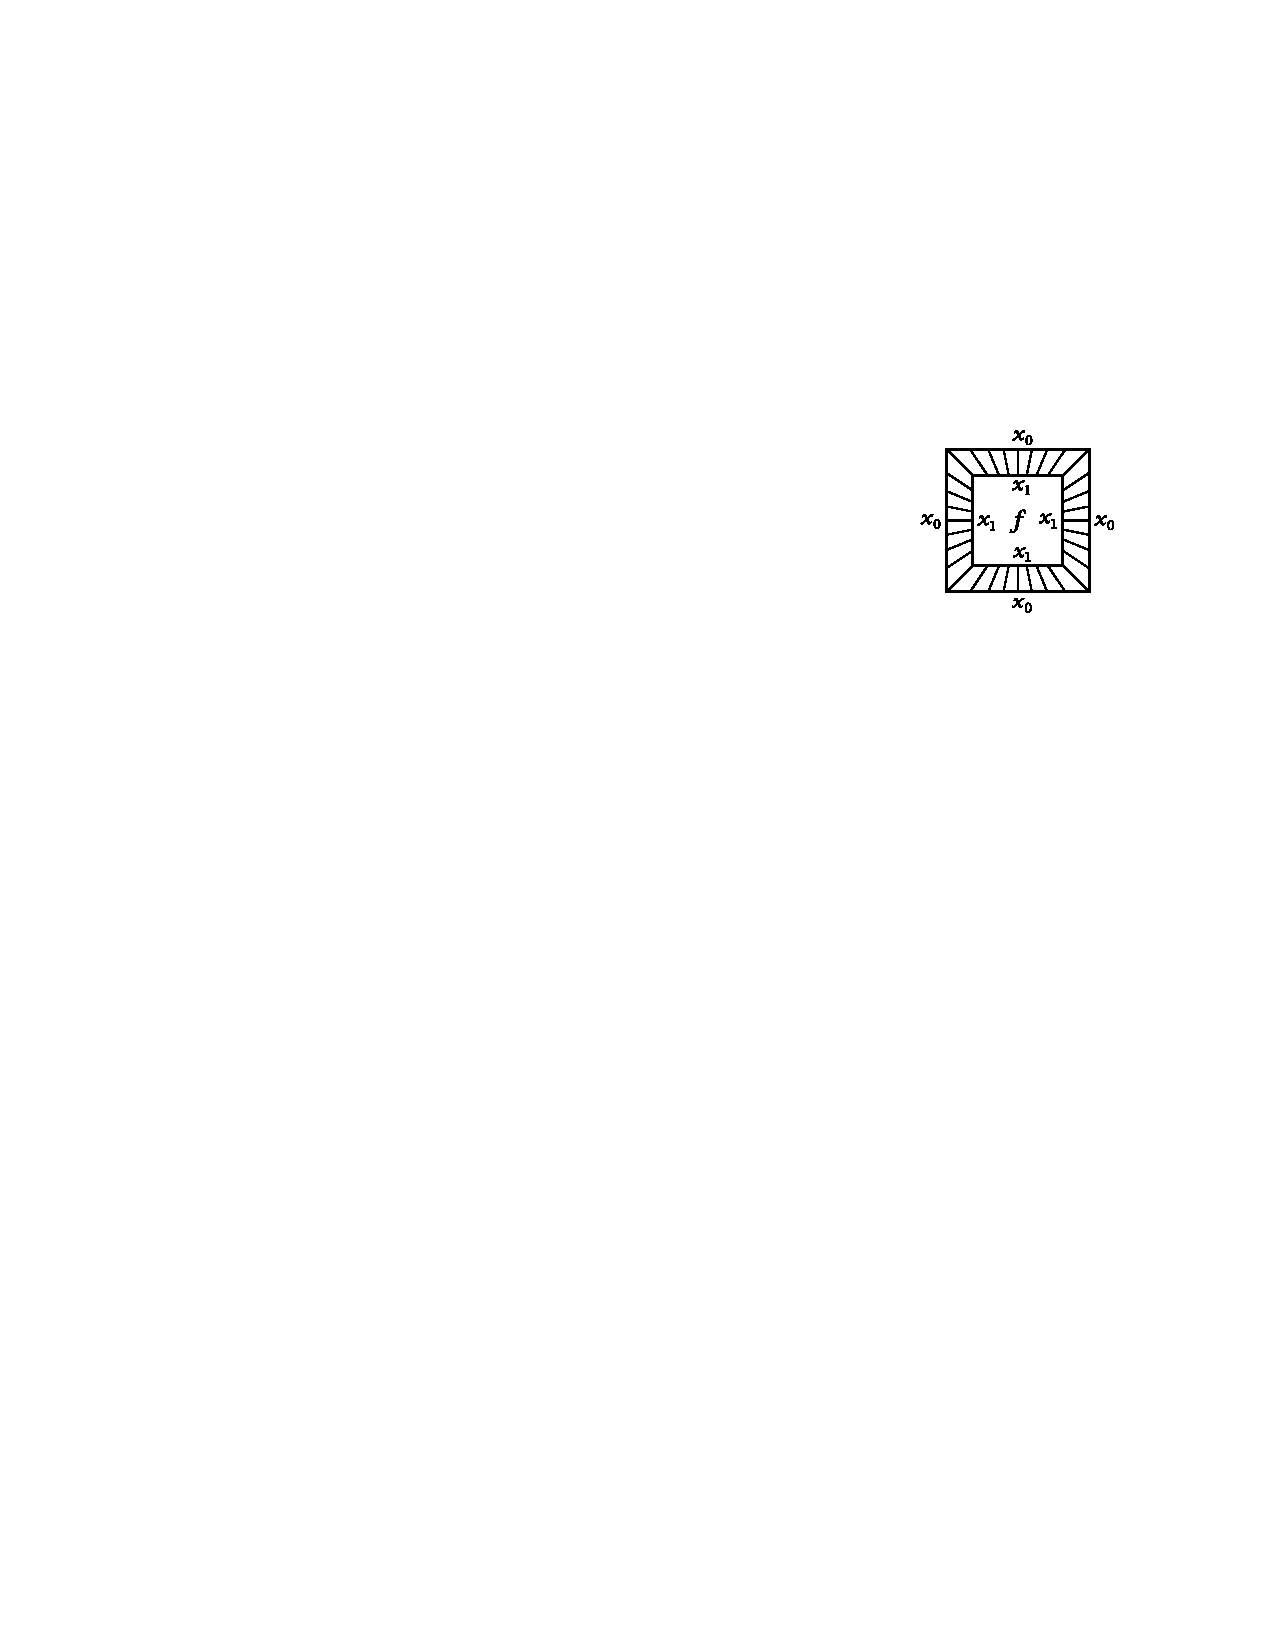
\includegraphics{3}
\end{center}
\end{frame}
\begin{frame}
\frametitle{\insertsection}
\framesubtitle{\insertsubsection}
\only<1>{Гомотопии $\gamma$ или $ f$ в отображениях связывающих
$\partial I$ или $\partial I^n$, соответственно, влекут
гомотопию $\gamma f$ в отображениях $(I^n,\,\partial I^n)\to 
(X,\,x_0)$. Ещё три важных свойства:
\begin{enumerate}
	\item $\gamma (f+g) \simeq \gamma f +\gamma g$,
	\item  $(\gamma \eta) f \simeq \gamma (\eta f)$,
	\item $1 f \simeq f$, где 1 обозначает тривиальный
		путь.
\end{enumerate}}
Гомотопии 2 и 3 очевидны. Для 1, мы сперва деформируем $f$ и
$g$ так, чтобы они были постоянными на правой и левой сторонах
$I^n$, соответственно. Получившиеся отображения мы можем
назвать $f+0$ и $0+g$, затем мы вырезаем все более широкий
средний кусок от $\gamma(f+0)+\gamma(0+g)$, пока это не
превратится в  $\gamma(f+g)$:
\begin{center}
	\includegraphics<2>[scale=0.7]{4}
\end{center}
\end{frame}
\begin{frame}
\frametitle{\insertsection}
\framesubtitle{\insertsubsection}
Явная формула для этой гомотопии:
\begin{multline*}
	h_t(s_1,\,s_2,\ldots,\,s_n)=\\= \begin{cases}
		\gamma(f+0)\left( (2-t)s_1,\,s_2,\ldots,\,s_n
		\right), & s_1 \in \left[ 0,\,\frac{1}{2} \right], \\
		\gamma(0+g)\left( (2-t)s_1+ t-1,\,s_2,\ldots
	,\,s_n\right), & s_1 \in \left[ \frac{1}{2},\,1 \right]. 
	\end{cases}
\end{multline*} 
Отсюда имеем $\gamma(f+g)\simeq \gamma(f+0)+\gamma(0+g)
 \simeq \gamma f +\gamma g$.
\end{frame}
\begin{frame}
\frametitle{\insertsection}
\framesubtitle{\insertsubsection}
Если мы определим преобразование смены базовой точки
$\beta_\gamma\colon \pi_n(X,\,x_1)\to \pi_n(X,\,x_0)$ как
$\beta_\gamma \left( [f] \right) =[\gamma f]$, то, т.\:к.
$\gamma(f+g)\simeq \gamma f +\gamma g$, то $\beta_\gamma$ ---
гомоморфизм.
\uncover<2->{В то же время из условий  $(\gamma \eta)f \simeq
 \gamma(\eta f)$,  $1 f\simeq f$ следует, что  $\beta_\gamma$ ---
изоморфизм с обратным элементом  $\beta_{\overline{\gamma}}$, где
$\overline{\gamma}$ это обратный к $\gamma$ путь,
$\overline{\gamma}=\gamma(1-s)$.}
\uncover<3->{Поэтому, если $X$ линейно связное пространство, различные базовые точки одного и того же
пространства доставляют нам изоморфные группы $\pi_n(X,\,x_0)$,
что может быть кратко записано как $\pi_n(X)$.}
\end{frame}
\end{document}
